\section{$e$-Funktion}\label{sec:e-Funktion}
Die E-Funktion ist einen Unterart der Exponentialfunktion (\ref{sec:Exponentialfunktionen}) sie hat, anders als eine Exponentialfunktion, einen belibige Zahl als Basis. Die Basis einer $e$-Funktion ist die eulischere Zahl $e$. 
\subsection{Entstehung von $e$} \label{sec:e-Funktion/Entstehung von e}
Die Entstehung von $e$ ist ein Grenzwertprozess...
%ToDo Entstehung von e
\subsection{Ableiten der $e$ Funktion}\label{sec:e-Funktion/Ableiten der e Funktion}
Die besonderheit bei $e$-Funktionen ist, dass die Differenzierte und Integrierte Funktion jeweils immer gleich ist. 
%ToDo Hier fehlen Informationen über das Integrieren und Differenzieren
\subsubsection{Faktorregel} 
Ähnlich wie bei dem normalen Ableiten bei einer ganzrationalen Funktion lässt sich hier die Faktorregel anwenden.
%ToDo Hier fehlen Informationen bezüglich des Ableitens und Differenzieren
\subsection{Umformung von der normalen Exponentialfunktion zu der E-Funktion}
Da sich die $e$-Funktion besonders gut differenzieren und integrieren lässt, nutzt man diese, um Sachverhalte darzustellen. Hierfür formt man die normale Exponentialfunktion so um, dass man sie als $e$-Funktion schreiben kann. Hierfür ist es relevant die Bedeutung der folgenden Normalform zu kennen. 
\subsubsection{Normalform}
\begin{align*}
	f(x)=a\cdot e^{k\cdot x+d}+c
\end{align*}
\geogebra{https://www.geogebra.org/m/bkar24wm}

\subsubsection{$a$ - Streckfaktor}
Der Faktor $a$ ist bestimmt die Streckungs/Stauchungs des Graphen. Wird dieser negativ, so wird der Graph an der $X$-Achse gespiegelt. Der Grund hierfür ist, dass ist $a$ negativ, werden die gesamten Werte des Graphen ebenfalls negativ. 
%ToDo Hier fehlt ein Graph mit einem Vergleich
\begin{figure}[h!]
\centering
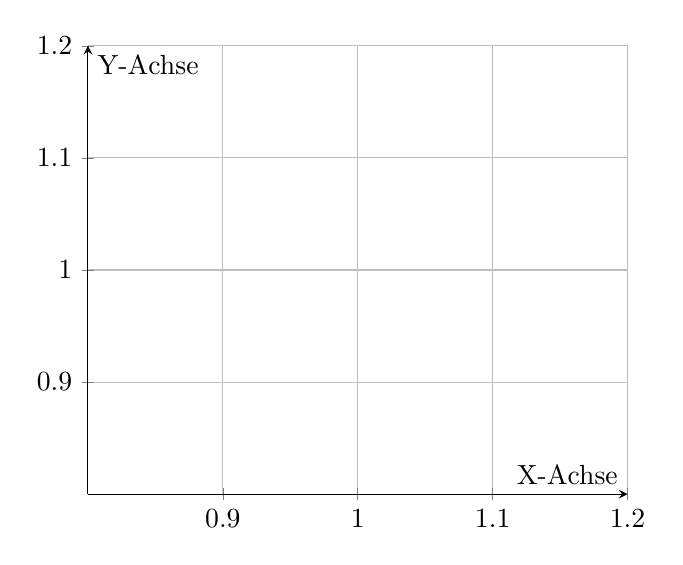
\begin{tikzpicture}
\begin{axis}[
    title={},
    xlabel={X-Achse},
    ylabel={Y-Achse},
    axis lines=middle, % Zentriert die Achsen
    xmin=1, xmax=1, % Setzt die Grenzen für die X-Achse
    ymin=1, ymax=1, % Setzt die Grenzen für die Y-Achse
    grid=major, % Fügt ein Hauptgitter hinzu
]
\end{axis}
\end{tikzpicture}
\caption{}
\end{figure}

\pagebreak
\subsubsection{$k$ - Koeffizent}
Der Faktor $k$ ist ähnlich wie $a$ und bestimmt die Streckung und Stauchung des Graphen, allerdings wird der Graph an der $Y$-Achse gespiegelt, sobald dieser negativ wird. Dies wird begründet durch 
Die Begründung hierfür ist, dass wenn eine Zahl für $k$ eingesetzt wird, bestimmt $k$ wie oft $x$ multipliziert wird. Hierdurch erreicht der Graph schneller die selben $Y$-Wert für $k>0$. Ist $k<0$, so kehrt sich der Graph um aufgrund der Negätivität von $k$. Werden nun postive Werte für $x$ eingesetzt, so entstehen hierraus immernoch negative Zahlen, denn $-$ mal $+$ ergibt $-$. Somit werden die gleichen $Y$-Werte wie im Positiven erricht, jedoch im Negativen.
%ToDo Hier fehlt ein Graph mit einem Vergleich
\begin{figure}[h!]
\centering
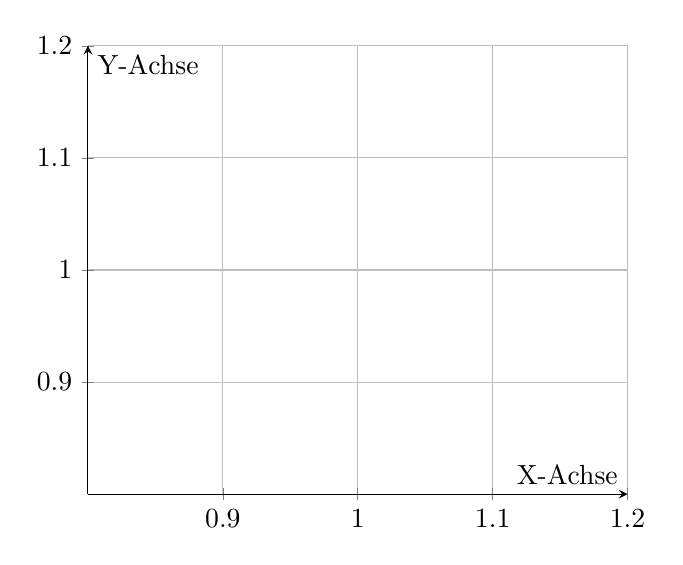
\begin{tikzpicture}
\begin{axis}[
    title={},
    xlabel={X-Achse},
    ylabel={Y-Achse},
    axis lines=middle, % Zentriert die Achsen
    xmin=1, xmax=1, % Setzt die Grenzen für die X-Achse
    ymin=1, ymax=1, % Setzt die Grenzen für die Y-Achse
    grid=major, % Fügt ein Hauptgitter hinzu
]
\end{axis}
\end{tikzpicture}
\caption{}
\end{figure}
\pagebreak
\subsubsection{$d$ - $X$-Achsenverschiebung}
Die Variable $d$ gibt die $X$-Achsenverschiebung an. Sei $d>0$ verschiebt sich der Graph nach links, andernfalls für $d<0$ verschiebt sich der Graph nach rechts. 
%ToDo Hier fehlt ein Graph mit einem Vergleich
\begin{figure}[h!]
\centering
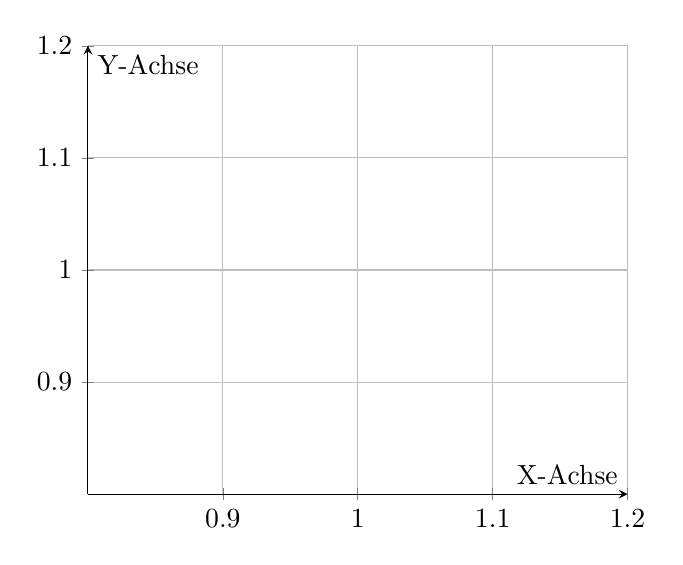
\begin{tikzpicture}
\begin{axis}[
    title={},
    xlabel={X-Achse},
    ylabel={Y-Achse},
    axis lines=middle, % Zentriert die Achsen
    xmin=1, xmax=1, % Setzt die Grenzen für die X-Achse
    ymin=1, ymax=1, % Setzt die Grenzen für die Y-Achse
    grid=major, % Fügt ein Hauptgitter hinzu
]
\end{axis}
\end{tikzpicture}
\caption{}
\end{figure}

\pagebreak
\subsubsection{$c$ - $Y$-Achsenverschiebung}
Der Summand $c$ bestimmt die $Y$-Achsenverschiebung. Dies ist begründet durch die Tatsache, dass wenn ein Summand zu $x$ addiert wird, dieser immer um $c$ nach oben verschoben ist. 
%ToDo Hier fehlt ein Graph mit einem Vergleich
\begin{figure}[h!]
\centering
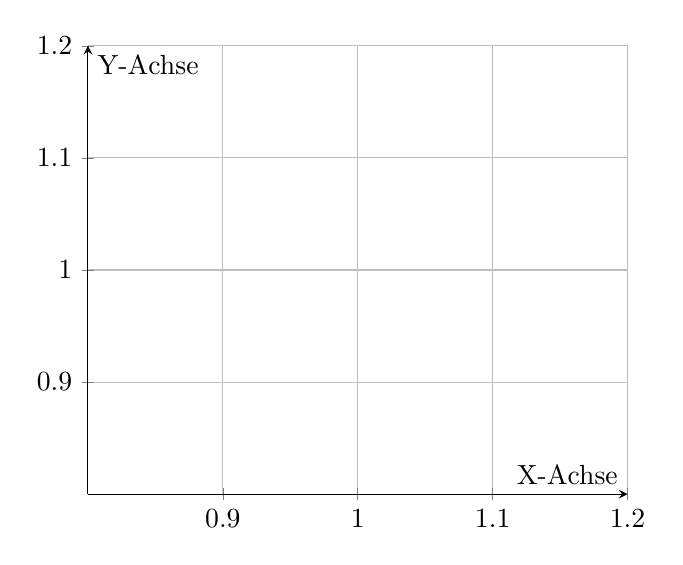
\begin{tikzpicture}
\begin{axis}[
    title={},
    xlabel={X-Achse},
    ylabel={Y-Achse},
    axis lines=middle, % Zentriert die Achsen
    xmin=1, xmax=1, % Setzt die Grenzen für die X-Achse
    ymin=1, ymax=1, % Setzt die Grenzen für die Y-Achse
    grid=major, % Fügt ein Hauptgitter hinzu
]
\end{axis}
\end{tikzpicture}
\caption{}
\end{figure}

